\documentclass[14pt]{beamer}


\setbeamercolor{item projected}{bg=black}
\setbeamertemplate{itemize items}[circle]
\graphicspath{{Figures/}}
\mode<presentation>
{
%  \usetheme{Boadilla}
  \usetheme{CambridgeUS}
  % or ...

  \setbeamercovered{transparent}
  % or whatever (possibly just delete it)
}


%\usepackage[english]{babel}
% or whatever

%\usepackage[latin1]{inputenc}
% or whatever
\usepackage{amsmath,amssymb,latexsym,epsfig,graphicx,psfrag,pstricks, fancybox, ulem}
\usepackage{booktabs}
%\title{Seminar Presentation} % (optional, use only with long paper titles)
\subtitle{Modelling and analysis of a financial market with slow and fast trading agents acting on time-delayed market information}
\title{Master's Thesis}
\author{Halfdan Rump}
\date{February 5 2014} % (optional, should be abbreviation of conference name)
\institute{Waseda GRS-FSE} % (optional, but mostly needed)

\newenvironment{changemargin}[2]{% 
  \begin{list}{}{% 
    \setlength{\topsep}{0pt}% 
    \setlength{\leftmargin}{#1}% 
    \setlength{\rightmargin}{#2}% 
    \setlength{\listparindent}{\parindent}% 
    \setlength{\itemindent}{\parindent}% 
    \setlength{\parsep}{\parskip}% 
  }% 
  \item[]}{\end{list}} 



\begin{document}

\begin{frame}
  \titlepage
\end{frame}





\section{Introduction}
\begin{frame}
\tableofcontents[currentsection]
\end{frame}

\begin{frame}{Background and motivation}
A few fact about modern financial markets:
\begin{itemize}
	\item Humans trade against software algorithms (the machines) 
	\item Humans are slow but complex, whereas algorithms are fast, but (relatively) simple
	\item Fast crashes (flash crashes) has become a problem in recent years
\end{itemize}
\end{frame}

\begin{frame}{Related work}
Models for human/machine system must be developed. Previous work:
\begin{description}
	\item[Analysis of market data] Works analyzing real market data for flash crashes and
	\item[Models of markets] Works that divide agents into two groups: \textbf{slow} and \textbf{fast} traders
\end{description}
All discovered works in the field are recent (published 2013, or yet unpublished).
\end{frame}

\begin{frame}{Key ideas in proposed model}
\begin{description}
\item[Delayed market information] All information exchanged between agents and the market is delayed
\item[Agents with arbitrary time delays] Agents are not just \textit{fast} or \textit{slow}, but have \textbf{arbitrary} delays
%\i tem[Full-fledged MAS model] Agents with various strategies and different delays.
\end{description}
\end{frame}

\begin{frame}{Research goal}
\begin{block}{Market stability and agent speed}
Investigate how the behavior (e.g. stable, crash, etc.) of a simulated financial market changes when the latency of the traders change
\end{block}
Very open research, but the first steps in a new field must necessarily be somewhat exploratory.
\end{frame}


%\begin{frame}{Methodology}
%
%\begin{itemize}
%content...
%\end{itemize}
%\end{frame}






\section{Model}
\begin{frame}
\tableofcontents[currentsection]
\end{frame}

\begin{frame}{Market model}
\begin{center}
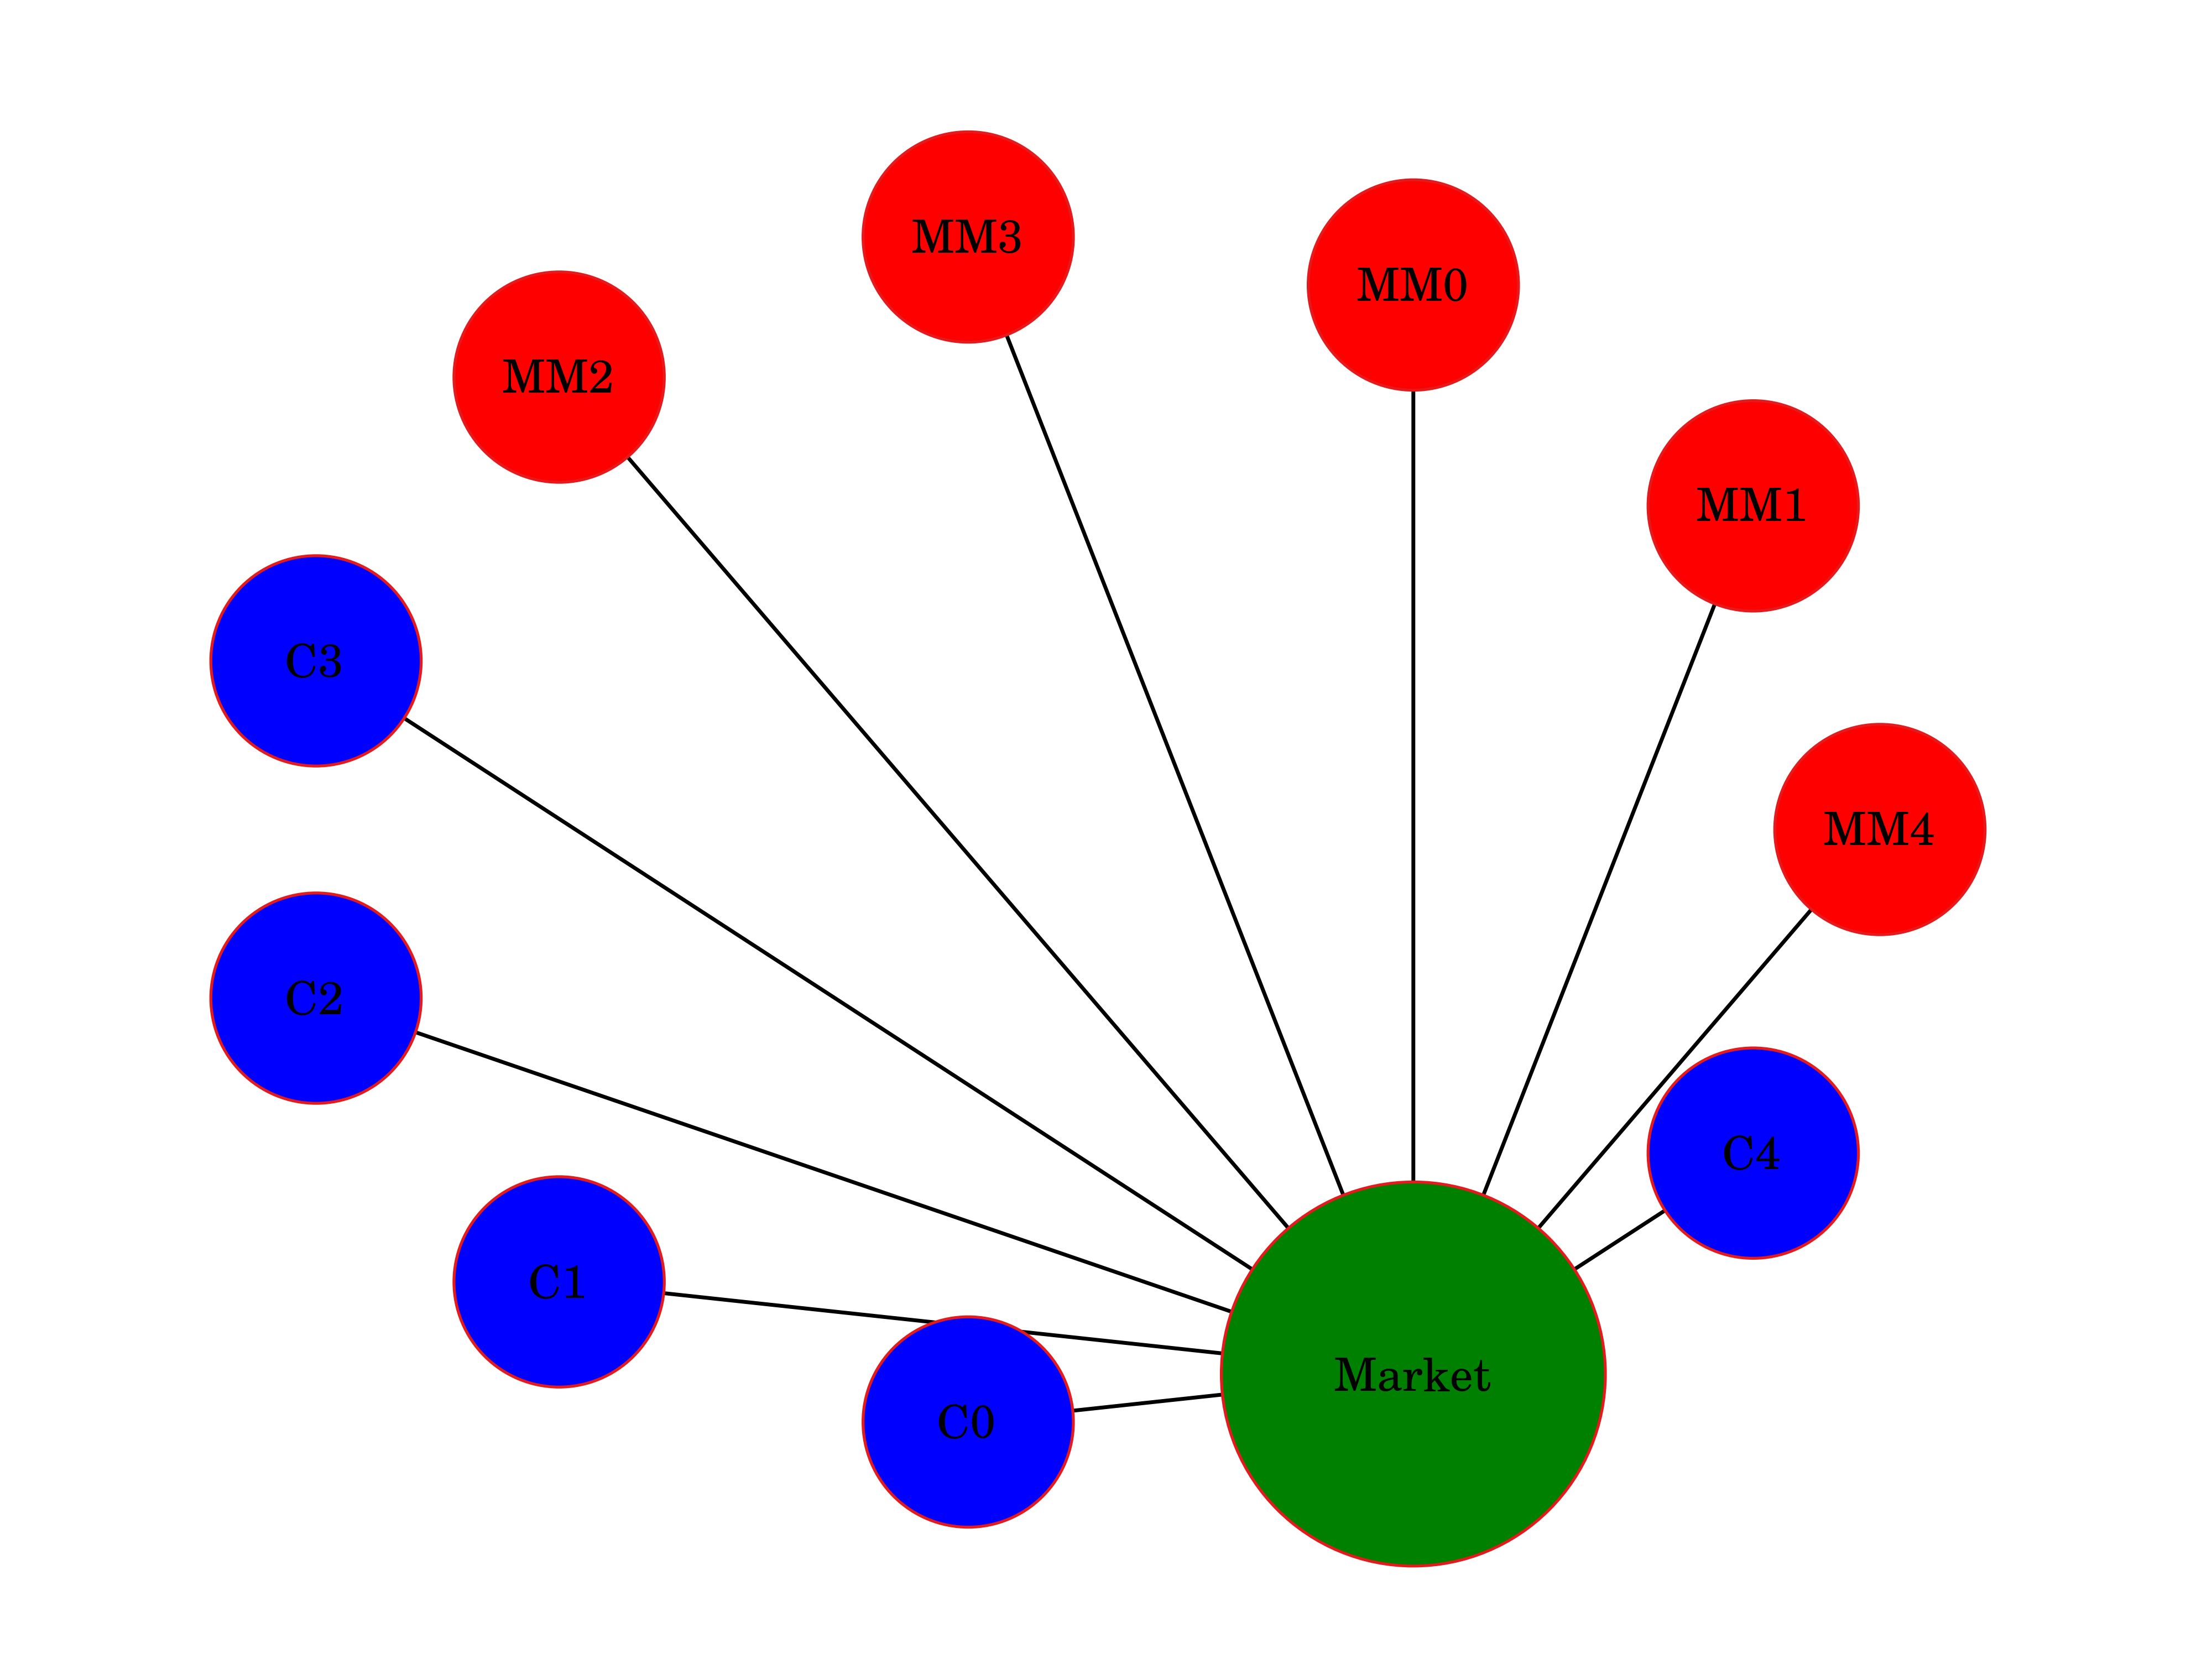
\includegraphics[width=0.7\textwidth]{graph.png}
\end{center}
\end{frame}

\begin{frame}{Model components}
\begin{itemize}
\item Market and order book
\item Stock
\item Agents
\item Messages
\end{itemize}
\end{frame}

\begin{frame}{Messages}
Information travels from agents to market in different kinds of messages
\begin{itemize}
\item Market information
\item Orders
\item Receipts
\item Cancellations
\end{itemize}
\textit{All messages have a non-zero travel time}
\end{frame}

\begin{frame}{Stock}
A single stock is traded at the market.
\begin{description}
\item[Fundamental price] The ``\textit{true}'' value of the stock
\item[Traded price] The price at which the stock is currently traded
\end{description}
\end{frame}


\begin{frame}{Agents}
\begin{itemize}
\item Slow traders (ST)
\item Fast traders (High Frequency Traders, HFT)
\begin{itemize}
\item Market makers (MM)
\item Simple chartists (SC)
\end{itemize}
\end{itemize}
\end{frame}



\begin{frame}{Slow traders}
\begin{block}{Slow traders model human traders}
They know the \textbf{true} value of the fundamental, \textit{but with a large delay}
\end{block}
The slow traders submit orders in order to \textit{move the trade price towards the true price}.
\end{frame}


\begin{frame}{Simple chartists}
\begin{block}{The chartists use a simple moving average strategy}
They calculate the moving from the delayed best buy and sell prices. 
\end{block}
The chartist detects a trend if the moving average calculated over $H_c$ rounds differs more than $\gamma_c$ ticks from the currently traded price.
\end{frame}

%\begin{frame}{Chartist example 1}
%\begin{center}
%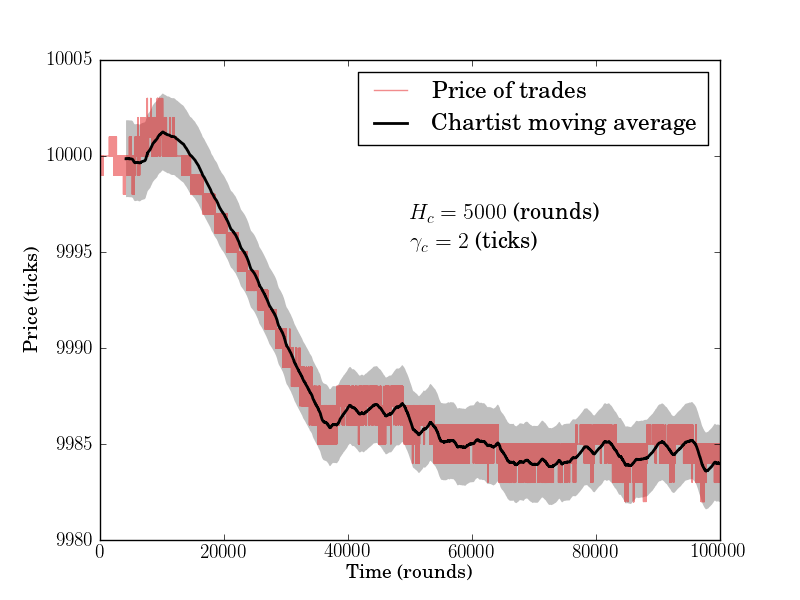
\includegraphics[width=0.7\textwidth]{chartist/b.png}
%\end{center}
%\end{frame}

\begin{frame}{Chartist example}
\begin{center}
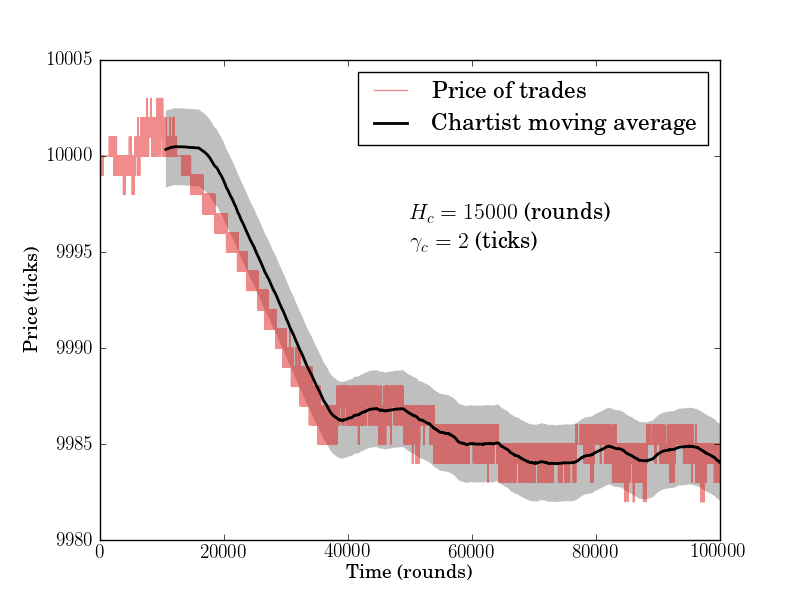
\includegraphics[width=0.7\textwidth]{chartist/h.png}
\end{center}
\end{frame}



\begin{frame}{Market makers}
\begin{block}{Market makers keep constant buy and sell orders}
The market maker tried to follow the best buy/sell prices to stay competitive.
\end{block}
The market maker has a minimum-spread parameter, $\theta$.
\end{frame}

\begin{frame}{Market maker case 1}
\begin{center}
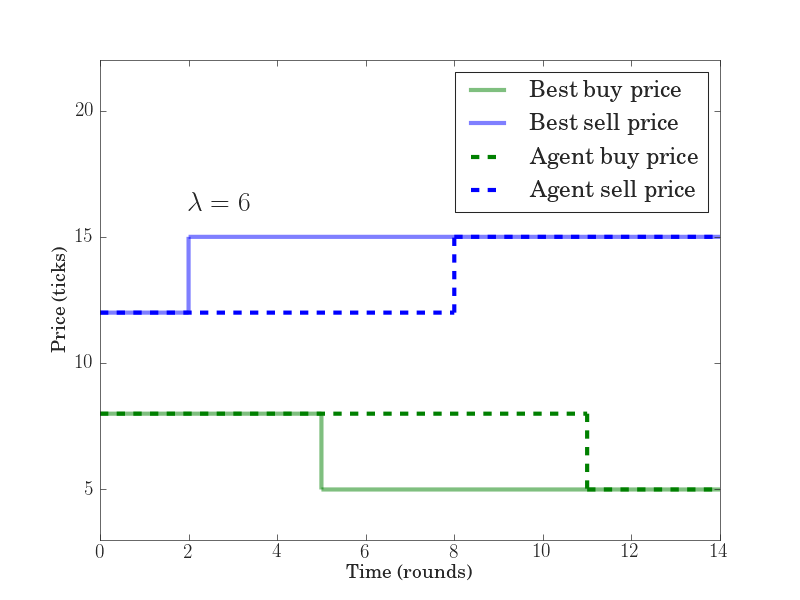
\includegraphics[width=0.7\textwidth]{marketmaker/a.png}
\end{center}
\end{frame}




\section{Experiments}
\begin{frame}
\tableofcontents[currentsection]
\end{frame}

\begin{frame}{Important model parameters}
The model has many parameters. The most important ones are:
\begin{itemize}
\item The average latency of chartists and of market makers, $\lambda$
\item The number of fast traders
\end{itemize}
\end{frame}


\begin{frame}{Simulating bad news}
\begin{block}{Shock to the fundamental}
How does the market react when the true price of the stock suddenly drops?
\end{block}
\end{frame}

\begin{frame}{A market with bad news}
\begin{center}
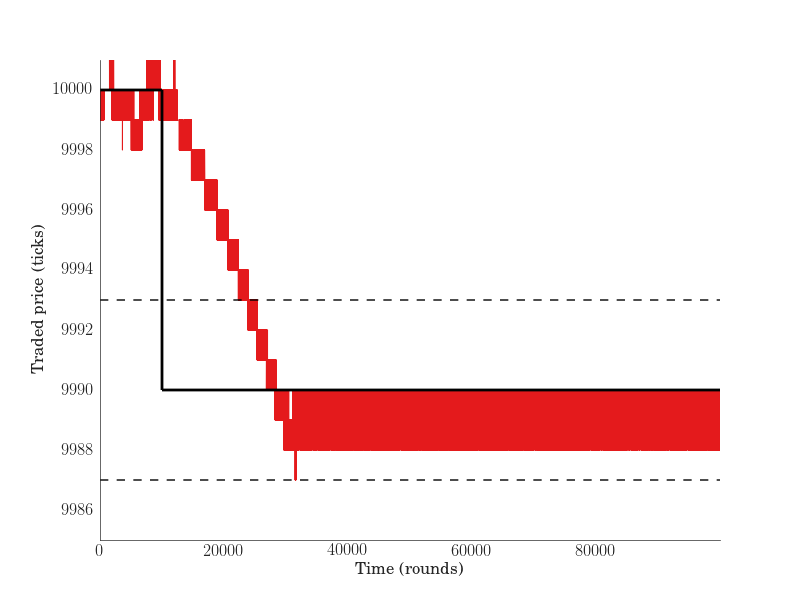
\includegraphics[width=0.7\textwidth]{market_cases/a_stable_within_margin.png}
\end{center}
\end{frame}

\begin{frame}{}
\begin{block}{We want to determine how the model behavior changes with the parameters}
A genetic algorithm was used to search the parameter space. Four fitness measures were defined in order to quantify the model behavior.
\end{block}
\end{frame}

\begin{frame}{Exploring model behavior with inverse simulation}
A genetic algorithm was used to find parameters causing \textbf{stable markets}. Four measures for model fitness were defined:
\begin{small}
\begin{description}
\item[Overshoot] Used to find \textbf{market crashes}
\item[Response time] Used to measure market reaction speed to \text{bad news}
\item[Price flickering] Standard deviation of trade prices)
\item[Time to become stable] the traded price must stay within a certain range of the true price)
\end{description}
\end{small}
\end{frame}

\begin{frame}{Stable market}
\begin{center}
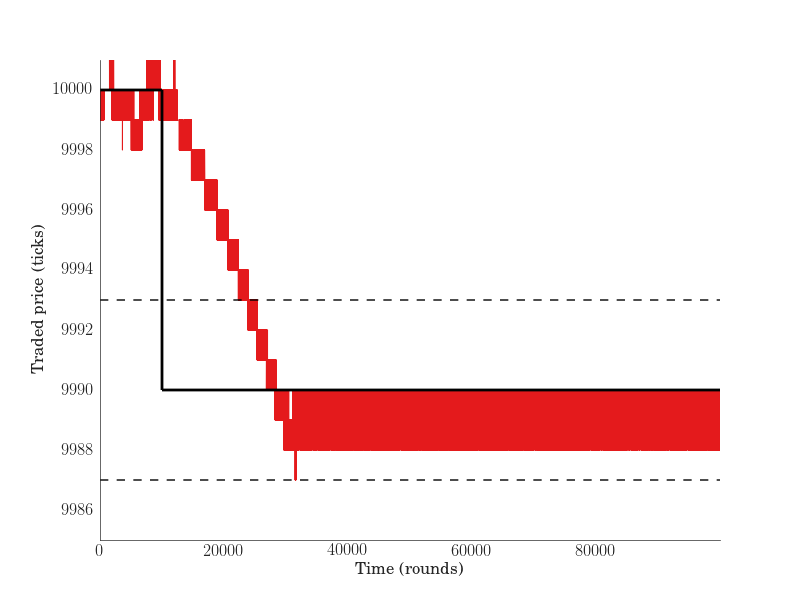
\includegraphics[width=0.6\textwidth]{market_cases/a_stable_within_margin.png}
\end{center}
The genetic algorithm was instructed to search for such markets.
\end{frame}

 
\begin{frame}{Market with large overshoot}
\begin{center}
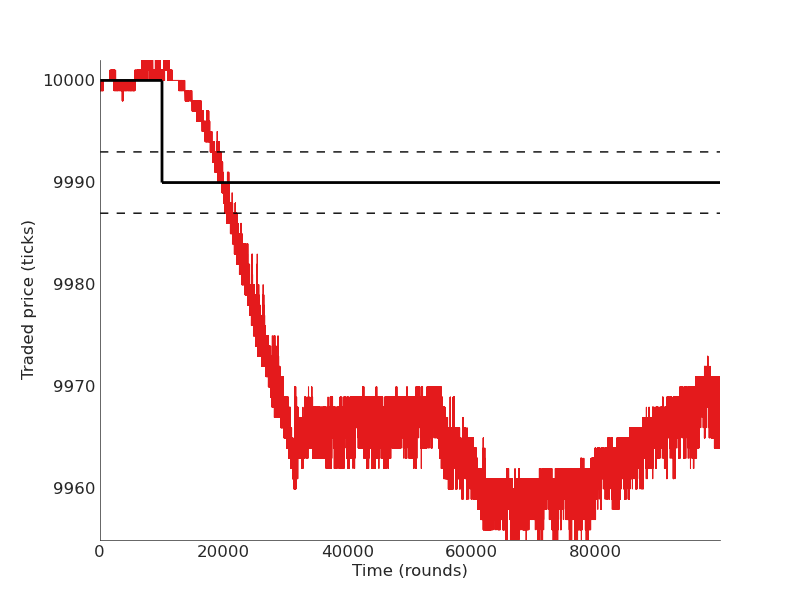
\includegraphics[width=0.7\textwidth]{market_cases/f_crash.png}
\end{center}
\end{frame}

\begin{frame}{Market with large price flicker}
\begin{center}
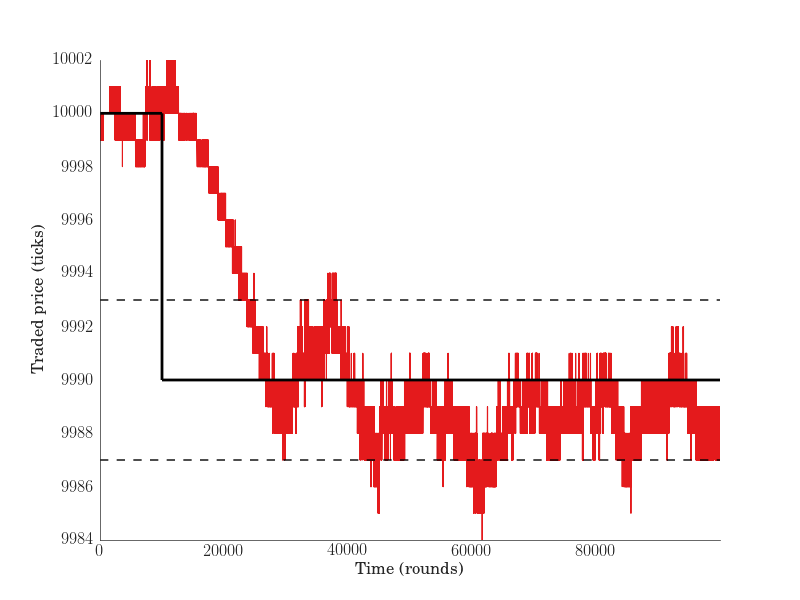
\includegraphics[width=0.7\textwidth]{market_cases/b_flicker_but_mostly_within_margin.png}
\end{center}
\end{frame}





	
\section{Results}

\subsection{Evolution of fitness and parameters}
\begin{frame}
\tableofcontents[currentsection]
\end{frame}

\begin{frame}{Overshoot}
The genetic algorithm found markets with a small overshoot, but which were also slow.
\begin{center}
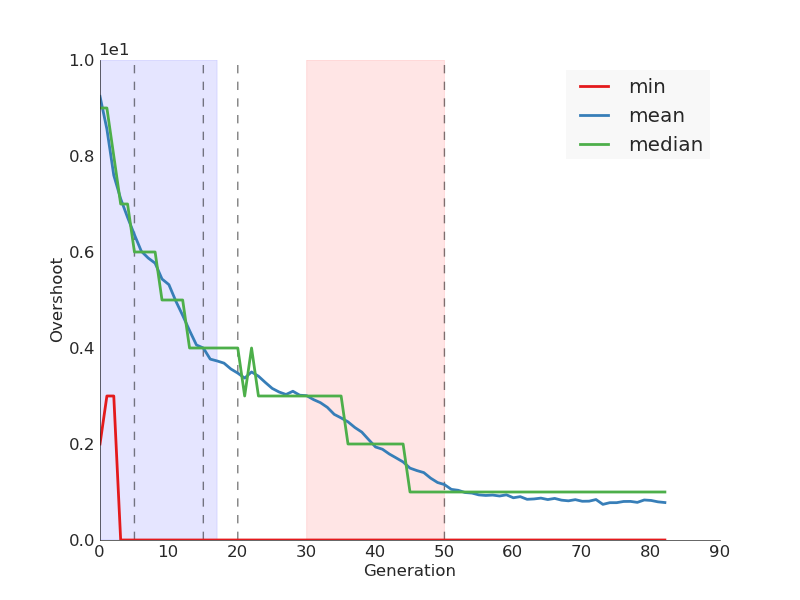
\includegraphics[width=0.4\textwidth]{evolution/overshoot.png}
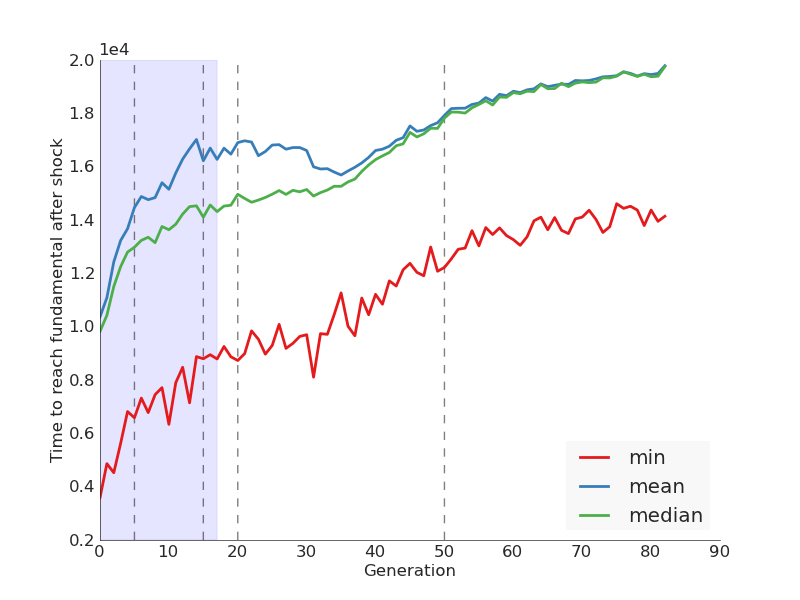
\includegraphics[width=0.4\textwidth]{evolution/time_to_reach_new_fundamental.png}
\end{center}
\end{frame}

\begin{frame}

\end{frame}

\begin{frame}{Speed/stability trade-off}
\begin{block}{}
The evolution of the fitness and parameters illustrates a trade-off between maket stability and the response time of the market: Stable market are also slower.
\end{block}
What parameters cause this behavior?
\end{frame}


\begin{frame}{Number of market makers}
The GA selects towards more market maker and slower agents
\begin{center}
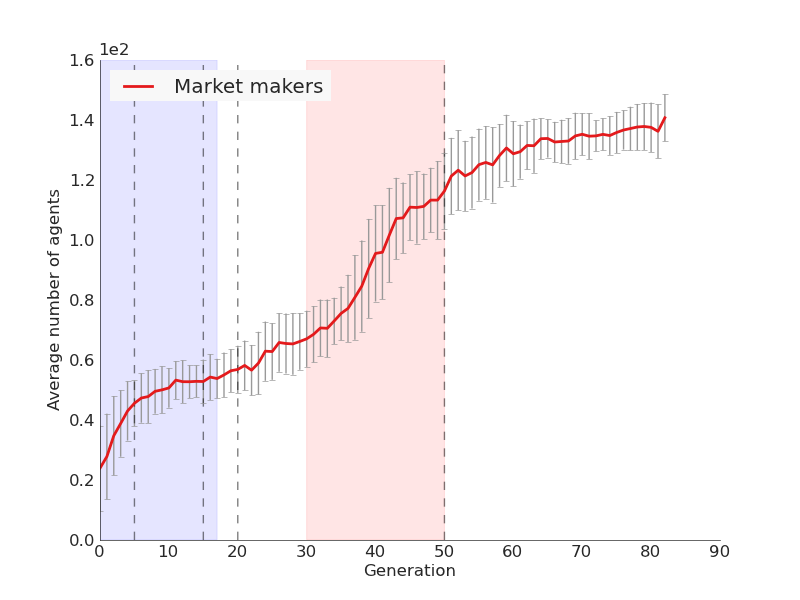
\includegraphics[width=0.4\textwidth]{evolution/nAgents.png}
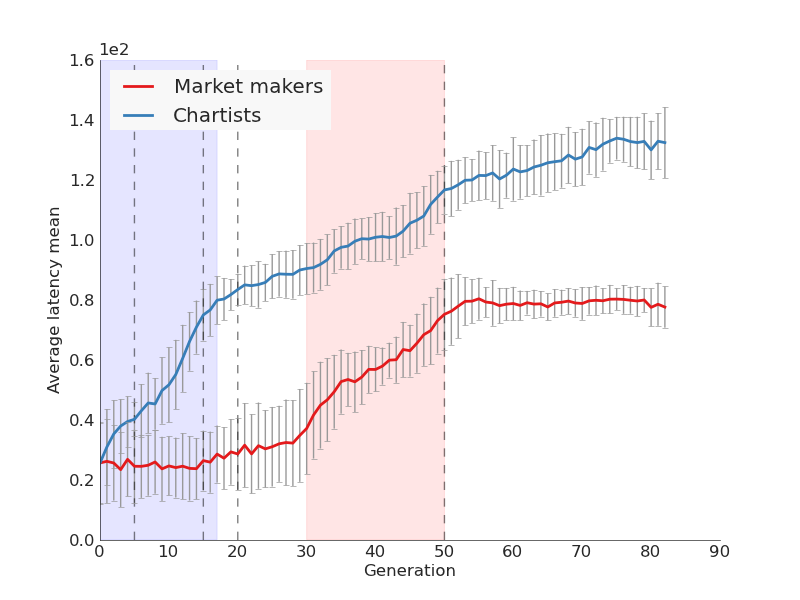
\includegraphics[width=0.4\textwidth]{evolution/latpars_mu.png}
\end{center}
\end{frame}



\subsection{Fitness/parameter correlations}
\begin{frame}
\tableofcontents[currentsubsection]
\end{frame}


\begin{frame}{Parameters and model behavior}
\textit{How does the speed of the agents affect the market behavior?}
\end{frame}

\begin{frame}{Chartist latency}
Faster chartists cause the market to have a larger overshoot:
\begin{center}
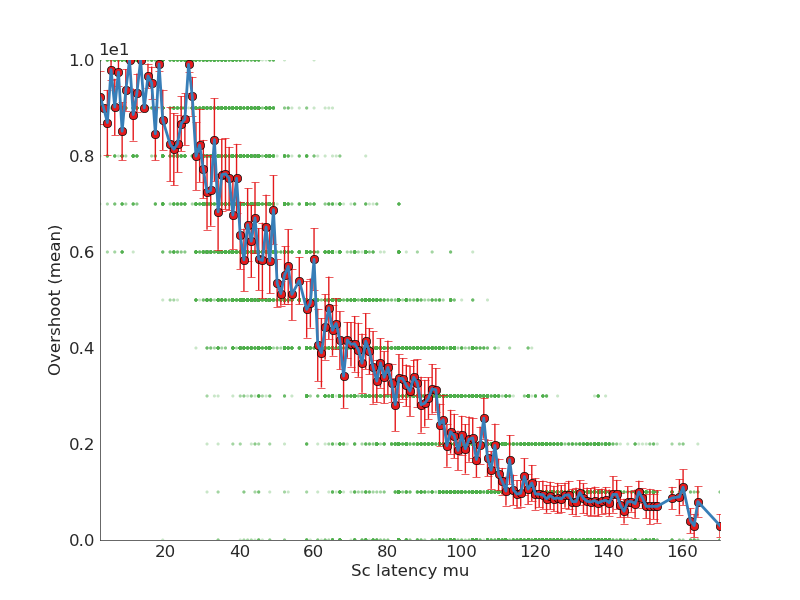
\includegraphics[width=0.7\textwidth]{scatter/sc_latency_mu__vs__overshoot(mean)_scatter.png}
\end{center}
\end{frame}

\begin{frame}{Market maker latence}
The number of market makers has a great deal to say:
\begin{center}
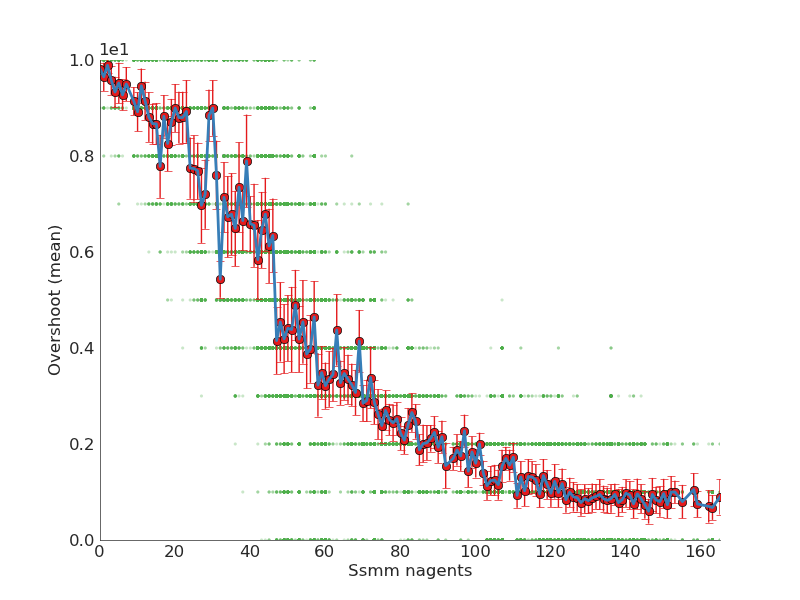
\includegraphics[width=0.7\textwidth]{scatter/ssmm_nAgents__vs__overshoot(mean)_scatter.png}
\end{center}
\end{frame}

%\begin{frame}{Number of chartists}
%...as has the number of chartists:
%\begin{center}
%\ includegraphics[width=0.7\textwidth]{scatter/sc_nAgents__vs__overshoot(mean)_scatter.png}
%\end{center}
%\end{frame}

\subsection{Parameter ratios}
\begin{frame}
\tableofcontents[currentsubsection]
\end{frame}

\begin{frame}{Latency ratio}
\textit{What happens when the chartists are faster than the market makers, or the other way around?}
\end{frame}

\begin{frame}{Overshoot}
\begin{center}
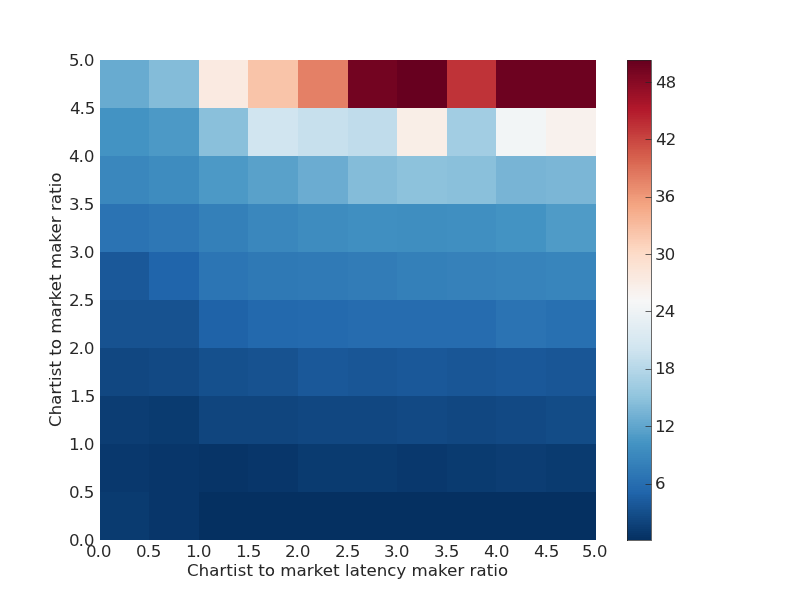
\includegraphics[width=0.6\textwidth]{ratio/overshoot.png}
\end{center}
Only markets with large chartist-to-market maker ratio crashed.
\end{frame}


%\begin{frame}{Log-overshoot}
%\begin{center}
%\ includegraphics[width=0.7\textwidth]{ratio/overshoot_log.png}
%\end{center}
%\end{frame}


\begin{frame}{Market response time}
\begin{center}
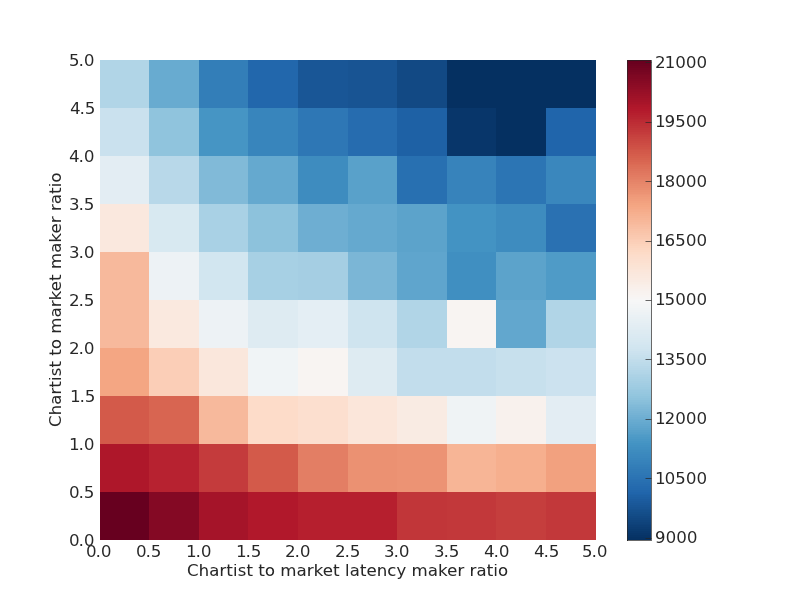
\includegraphics[width=0.6\textwidth]{ratio/time_to_reach_new_fundamental.png}
\end{center}
Markets with with a large chartist-to-market maker ratio responded faster.
\end{frame}

\begin{frame}{Latency is important}
\begin{enumerate}
\item Market makers stabilize the markets
\item Chartists increase price movements
\item The influence was \textit{larger} for \textit{faster} agents
\end{enumerate}
\end{frame}

\begin{frame}{Conditions for market crashes}
\begin{enumerate}
\item The market will only crash if \textit{both} chartists \textit{and} market makers are present.
\item The market was more likely to crash if the \textit{chartists were faster than the market makers}
\end{enumerate}
\end{frame}


\section{Conclusion}
\begin{frame}
\tableofcontents[currentsection]
\end{frame}

\begin{frame}{Conclusions}
\begin{description}
\item[Fast trader pros and cons] Fast agents both provided benefits to the market (faster response, lower price flickering), and caused some dangers (crashes, misvaluation)
\item[Stability/speed trade-off] The market was found to have a trade-off between speed and stability
\item[Relative agent latencies] The results illustrated the importance of allowing different agents to have different latencies.
\end{description}
\end{frame}



%We have more control over what simplifications we make than we have over events that we never observed.





%frame: black swans: some events are fundamentally unpredictable. Theories based on a few observations can never hope to predict these, as (only training data, no test data)




%frame: what I hope to be doing for the next two years. Artificial markets and HFT




%frame[advantages] - we can control conditions - we can repeat experiments - we can observe general trends and patterns

%frame[problems] - we need to simplify a lot - how do we simplify? - difficult to know if simplifications are OK or not - difficult to validate results obtained through simulation

%frame - emphasis on bottom up tinkering: create environment first, then play around - some top down approach is required when designing environment




\begin{thebibliography}{Bib}

\bibitem{mcgowan}
  Michael, J. McGowan,
  \emph{The Rise of Computerized High Frequency Trading: Use and Controversy}.
  Duke Law \& Technology Review,
  2012.
 \bibitem{izumi}
  K. Izumi, F. Toriumi, H. Matsui
  \emph{Evaluation of automated strategies using an artificial market}.
  Neurocomputing,
  2009.
  \bibitem{cincotti}
  S. Cincotti, S.M. Focardi, L. Ponta, M. Raberto, E. Scalas
  \emph{The waiting-time distribution of trading activity in a double auction artificial financial market}. Unpublished, 2011
  \bibitem{luca}
  M. De Luca, C. Szostek, J. Cartlidge, D. Cliff
  \emph{Studies of interactions between human traders and algorithmic trading systems}.
  Commissioned as part of the UK {Government's} Foresight Project, The Future of Computer Trading in Financial Markets--Foresight Driver Review--DR 13, 2011
  \bibitem{johnson}
  N. Johnson, G. Zhao, E. Hunsader, J. Meng, A. Ravindar, S. Carran, B. Tivnan
  \emph{Financial black swans driven by ultrafast machine ecology}.
  Submitted, 2012.
   

\end{thebibliography}

\begin{frame}{Market}
\begin{block}{Auction type}
The market uses a continuous double auction. Prices are always executed at the prices of the best standing market orders.
\end{block}
\end{frame}


\begin{frame}{Order book}
\begin{table}
\centering
\begin{tabular}{l|c|r}
Sell orders & Price & Buy orders\\
\midrule
22 & 9994 &\\
26 & 9993 &\\
13 & 9992 &\\
10 & 9991 &\\ 
{}&{}&{}\\
& 9988& 12\\
& 9987& 10\\
& 9986& 16\\
& 9985& 25\\
\end{tabular}
\end{table}
\end{frame}


\end{document}


